\chapter{Problem description}
\label{chp:problem-description}

Tribler's goal is to offer a YouTube-like experience with similar performance and ease of use.
All Tribler's features are implemented in a completely decentralized manner, not relying on any centralized component.

Numerous initiatives exist around these goals of re-decentralisation and performance.
However, none of them gathered any significant usage compared to the social media usage levels. 
For instance, YouTube features one billion unique monthly users \cite{mainka2014government} and there are 1.8 billion monthly active Facebook users \cite{sharma2016strategies}.

The problem is that the performance, usability, and features offered by decentralised alternatives are inferior when compared to the experience offered by central solutions.
Creating academically pure self-organising systems such as Tribler has proven to be notoriously difficult.
For example, the extensive list of 194 projects which all aim to create an alternative Internet experience using decentralisations shows the amount of years spent and lines of code produced \cite{redecentralize2016alternative}.
Most of these projects are abandoned and few of them have actual real-world usage.

\begin{figure}[!h]
	\makebox[\textwidth][c]{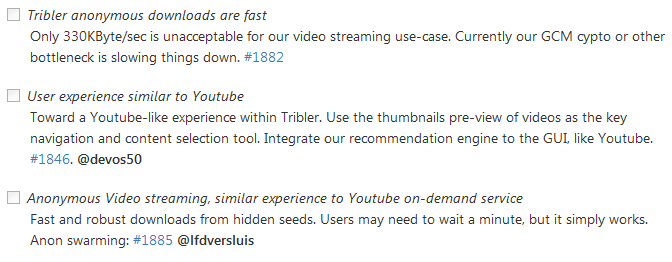
\includegraphics[width=\linewidth]{problemDescription/images/roadmap}}
	\caption{Three of the six uncompleted Tribler roadmap items.}
	\label{fig:tribler_roadmap}
\end{figure}

The Tribler project created a roadmap -- available on its GitHub repository -- to offer the same service, features, user experience, and performance as the YouTube video-on-demand service.
However, especially the poor performance of Tribler is hampering wide-spread adoption and usage. Figure~\ref{fig:tribler_roadmap} shows three of the six main uncompleted roadmap items.

\section{Key Performance Optimizations}

Tribler can be seen as a large and complex distributed system.
Metrics from OpenHUB show that Tribler, along with its components, features more than 169 thousand lines of code, received contributions from 111 unique contributors and took approximately 44 years of effort \cite{openhub2016tribler}.

In large and complex systems there are likely to be many performance issues present, often referred to as \emph{bottlenecks}.
J. M. Juran's Pareto principle admonishes that one should "Concentrate on the vital few, not the trivial many" \cite{ammons2004finding}. This principle is also known as the 80/20 rule.
Concretely, this means that resolving the vital bottlenecks yields the best diminishing returns, even for large systems such as Tribler.
After careful scrutiny it was decided that the most vital bottleneck to address, within the context of a nine month thesis, is Tribler's database I/O.

\section{Addressing Blocking I/O}
\label{sct:triblers_database_dependency}

The problem we address within this thesis is the underlying reason for poor performance and unacceptable user experience. 
Measurements dating back from 2013 indicate that Tribler's performance is I/O-bound \cite{pouwelse2014reduce}.
Especially with slow hard disks, but also with fast SSD storage the main performance bottleneck seems to be around database access.
With our focus on the fundamental issue we believe we can make a significant step forward in making decentralized technology able to compete with centralized solutions on large-scale usage.

\begin{figure}[!h]
	\makebox[\textwidth][c]{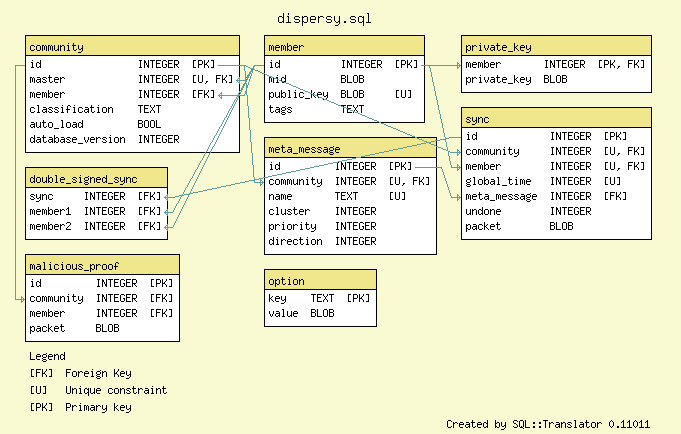
\includegraphics[width=\linewidth]{problemDescription/images/dispersy_database_schema}}
	\caption{The database schema of Dispersy, (source: Johan Pouwelse, 2013) \cite{pouwelse2013documentation}.}
	\label{fig:dispersy_database_schema}
\end{figure}

All information within Tribler is stored in a database for persistence and ease of use.
Information about the network i.e. peers, messages and authentication is stored in a separate database managed by the Distributed Permission System (Dispersy).
Dispersy is an elastic database system written in the Python programming language and uses SQLite as its underlying database engine.
It lies at the heart of Tribler, providing the means to discover peers and content in a decentralized way while offering security and anonymity.

Dispersy is fully decentralized with the exception of bootstrap servers.
It can run on systems with a large number of nodes, without any sever architecture needed \cite{dispersy2016dispersy, zeilemaker2013dispersy}.
All nodes perform the same algorithmic procedures and tasks and do not differentiate between any node i.e. all nodes are equal.

Furthermore, Dispersy provides one-to-one and one-to-many data dissemination mechanisms to forward data to nodes.
Eventually, all data will reach all nodes in the network, overcoming challenging network conditions.
The current overview of the database structure is presented in Figure~\ref{fig:dispersy_database_schema} (Johan Pouwelse, 2013).

These databases are becoming a key performance bottleneck \cite{pouwelse2014reduce}.
Back in May 2013 measurements indicated that Tribler read and wrote 660 Megabytes per hour to and from disk.
The next measurement in April 2014 showed this number was somewhat reduced to 623.
In May 2014 efforts were made to reduce this enormous amount of I/O; by batching database statements the number dropped to 538 megabytes per hour.

So far this metric has only been measured sporadically by hand, running Tribler for an arbitrarily amount of time and check the amount of I/O by using htop\footnote{\url{http://hisham.hm/htop/}}.
htop produces an overview similar to Figure \ref{fig:iotop_tribler_april_2014} (Johan Pouwelse, 2014).
Measurements to observe to which extent Dispersy is responsible for these numbers were never conducted, however it is strongly suspected by the Tribler developers that Dispersy is responsible for most of it.
Since 2014 no work or measurements have been done related to this issue.

\begin{figure}[!h]
	\makebox[\textwidth][c]{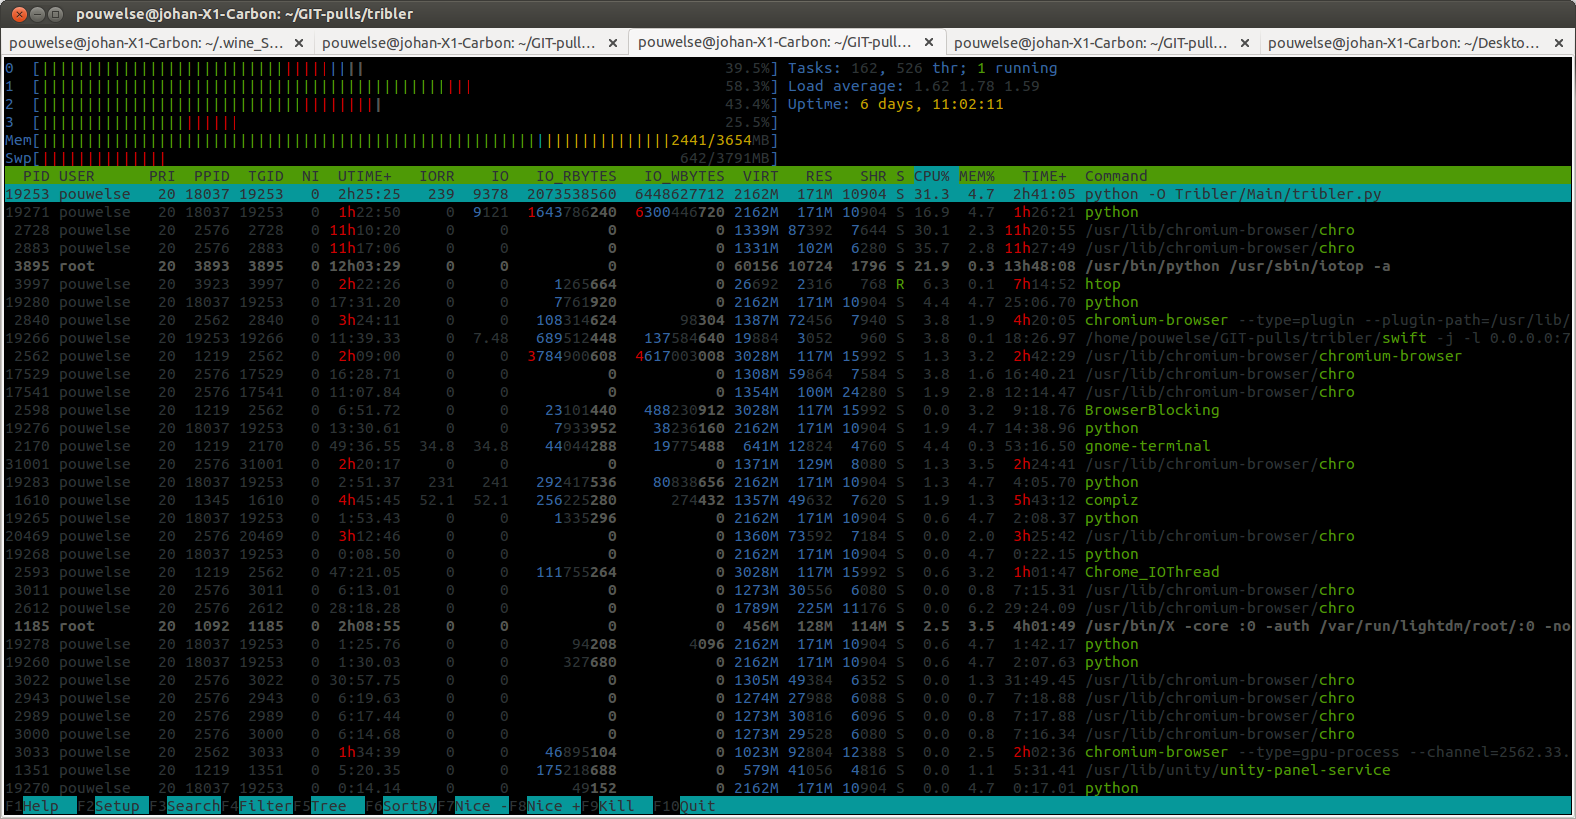
\includegraphics[width=0.9\paperwidth]{iointribler/images/iotop}}
	\caption{A screenshot of htop showing Tribler's I/O, (source: Johan Pouwelse, 2014 \cite{pouwelse2014reduce}).}
	\label{fig:iotop_tribler_april_2014}
\end{figure}

\subsection{Blocking I/O}
One of the main causes of Tribler's performance issues can be explained by the blocking behaviour of I/O.
Currently, Dispersy is deeply embedded into Tribler, running on the same (main) thread Tribler is running on.
Tribler, just like Dispersy, is written in the Python programming language.
In Python, a thread performing an I/O operation will block, causing all operations on the thread to suspend.
This means whenever Tribler or Dispersy performs I/O all functions of Tribler and Dispersy halt.
With the enormous amount of I/O Tribler is performing, this forms a huge limiting factor on the responsiveness and therefore performance of Tribler.

When a thread suspends, other threads can take over and perform operations, yet besides the main thread there are only two additional threads in Tribler: the Graphical User Interface (GUI) thread and the Dispersy endpoint thread.
As the name implies, the GUI is running on the GUI thread as the framework Tribler currently uses requires this.
Ironically, the Dispersy endpoint thread was introduced because of the blocking I/O behaviour.
Under heavy load, Dispersy drops incoming packets because it cannot keep up.
Processing packets is done on the main thread and as this thread frequently blocks, the buffers overflow causing packet loss.
These two threads do not saturate the available processing time offered by the main thread blocking, leading to wasting valuable CPU cycles.

Furthermore, Tribler has seen several changes to its code base including the addition of the MultiChain: Tribler's own Blockchain-like structure \cite{norberhuis2015multichain}.
This feature heavily relies on its database to store blocks and other information about the user and other peers.
Moreover, the MultiChain makes use of its own database rather than Dispersy's.
Norberhuis points out: \enquote{The information is stored in two places within Tribler and this could be eliminated. It would reduce the disk footprint and the amount of read/write transactions as only one database would have to be maintained. The I/O ineractions[sic] are a problem according to Tribler maintainers.} \cite{norberhuis2015multichain}, yet numbers on how much I/O the MultiChain generates are not presented.
This makes it hard to estimate Tribler's current I/O rates.

What's more, a feature called \enquote{credit mining} is currently in development that will also interact with the database of Tribler.
There are no metrics on the current situation of Tribler and it's hard if not impossible to estimate the impact of any addition to come.
Currently, there is a lack of insight in these metrics, or a lack of \emph{software performance engineering}, causing the exact extent of the problem to be unknown.

%\section{Asynchronous I/O}
%\label{sec:async-programming}

\section{A Lack of Software Performance Engineering}

\begin{figure}[!h]
	\makebox[\textwidth][c]{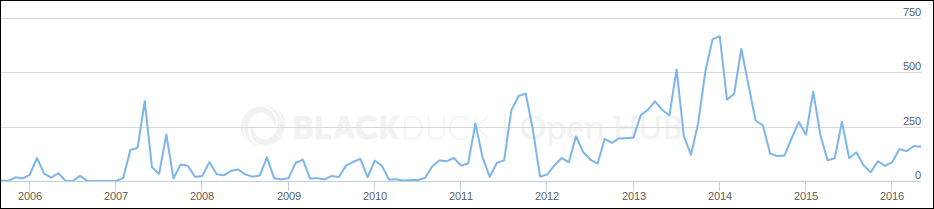
\includegraphics[width=\linewidth]{problemDescription/images/commits_openhub.png}}
	\caption{The distribution of commits on Tribler (source: OpenHUB, 2016 \cite{openhub2016tribler}).}
	\label{fig:commits_openhub}
\end{figure}

Nowadays, programs are evolving at a rapid speed and Tribler is no exception. 
Since 2005 Tribler is under continuous development, over seventeen thousands commits have been made, spanning more than a decade \cite{openhub2016tribler}.
The distribution of these commits can be seen in Figure~\ref{fig:commits_openhub}.
Code commits to fix bugs, refactor code, enhance or add functionality are pushed to the code repository of Tribler at a frequent rate.
It is important that software performance engineering is a part of this process: performance should not get compromised by changes, if any it should improve.
Naturally trade-offs can be made performance wise, but it should be done with a clear understanding of the consequences.

For the past three years, attempts have been made to monitor the performance, yet with little success.
The first attempt was to create probes using Systemtap\footnote{\url{https://sourceware.org/systemtap/}}.
System tap is a tool for \enquote{instrumenting the Linux kernel for analyzing performance and functional problems}, (Jacob et al. 2008) \cite{jacob2008systemtap}.
While some success was reported, this system is no longer being maintained nor functional.
After this, code was added to the Dispersy code base to track and log if a function was running longer than a fixed amount of time.
While this implementation does provide some insight, its workings are crude and only covers some of the functions present.
For instance, it cannot handle asynchronous constructions.
Tribler did not have any observation system integrated, leaving the development team in the dark regarding its performance.

It is apparent that there is a lack of software performance engineering in the development cycle of Tribler.
Performance has never been one of the priorities in Tribler's lifetime: only 6\% of all tickets on GitHub are (indirectly) related to performance based on their content.
To ensure performance will no longer degrade, realistic benchmarks need to be developed which Tribler can be tested with.
Changes can then be compared against the current code base, tracking important performance statistics such as the amount of I/O, run time of functions, throughput and responsiveness.
These benchmarks can then be integrated into a regression testing system which can be integrated in our Jenkins continuous integration system.
Using Jenkins, performance regression tests can run on every proposed change and at predetermined moments, allowing for a continuous updated overview of Tribler's performance metrics.

% https://github.com/Tribler/tribler/issues/15
% https://github.com/Tribler/tribler/issues/77
% experiment framework: https://github.com/Tribler/tribler/issues/114
% latency grpahs? https://github.com/Tribler/tribler/issues/119
% speed of streaming: https://github.com/Tribler/tribler/issues/134
% of course: https://github.com/Tribler/tribler/issues/3
% nightly runs: https://github.com/Tribler/tribler/issues/184
% extreme cpu ticket: https://github.com/Tribler/tribler/issues/197
% slow startup time ticket: https://github.com/Tribler/tribler/issues/255

\section{Realistic Benchmarks}
Directly related to the performance problem is the benchmark problem.
In order to improve user performance we require making assumptions about realistic use cases.
Each user has different usage patterns, hardware and network conditions, all affecting performance.
Creating several benchmarks testing realistic scenario's is required to accurately tune the system for real world usage.
At the same time, a benchmark cannot consume too much time.
Benchmarking is by nature time consuming \cite{huang2014performance}, however running long regression tests per commit will severely strain the development speed.

Therefore, it is important to create a reference benchmark which has a close resemblance to real world usage without consuming too much time.

\section{Objective and Research Questions}
\label{chp2:sct:objectives-research-questions}
The objective of this thesis is to improve the performance and responsiveness of Tribler and to introduce a regression testing system.
The verification of the performance regression testing system is done by focussing on removing Tribler's biggest bottleneck present: blocking database I/O.
By resolving this bottleneck, important metrics tracked by this regression testing system should show positive changes, indicating improvement.

The research presented in this thesis was carried out in cooperation with the Tribler team. 
The Tribler team consists of both staff members of the Technical University of Delft as well as Bachelor and Master students.
Based on the objectives of Tribler, this thesis aims to answer the main research question formulated below.\\

\textbf{Main Research Question:} How can we improve Tribler's performance, responsiveness and throughput?\\

To answer this main research question, we have defined three research questions below. Each of these research questions will be justified as why they contribute to the main research question.\\

\textbf{Research Question 1:} Can a system such as Tribler benefit from asynchrony?\\

To improve performance and responsiveness, parts of Tribler can be rewritten to become asynchronous.
By performing tasks asynchronously the performance and responsiveness of a program can improve.
However, an asynchronous approach can have its drawbacks. 
One of these drawbacks is that it requires a different mindset for the programmers as the whole call chain and structure of a program becomes different.
Identifying these drawbacks and deciding if the benefits outweigh the costs is necessary to prevent the current state from worsening. \\

\noindent
\textbf{Research Question 2:} How do we resolve Tribler's blocking database I/O problem?\\

As database I/O is currently the main bottleneck, we need to resolve it.
Tribler already has a framework integrated that is especially designed to handle I/O in a non-blocking way.
We require an approach that prevents us from reinventing the wheel while still solving the bottleneck at hand in an adequate manner.
Additionally, we need to make sure the order of database operations does not change as this may lead to inconsistencies.

Careful scrutiny is required to look at available solutions and their pros and cons.
A decision can then be made on the best course of action. \\

\noindent
\textbf{Research Question 3:} How do we incorporate software performance engineering into Tribler's development process to gain insight into performance statistics?\\

Currently, not a single developer has insight into how well Tribler performs and what impact changes have on Tribler in its current state.
To be able to conclude performance changes do not negatively impact the performance of Tribler, we can apply software performance engineering.
Software performance engineering focuses on introducing performance regression tests and benchmarks into the development cycle.
By making use of these regression tests, Tribler developers finally get insight into vital metrics which is desperately needed.\\


\section{Main Contributions}
The main contributions of this thesis are as follows.
First, we elaborate on the subject of multitasking and parallelization in the context of the Python programming language and provide arguments where asynchronous programming is preferred over synchronous programming, using Tribler as a case study.
We then resolve the vital I/O bottleneck currently present in Tribler using asynchrony and a multi-threaded approach.
This is done by introducing the Storm database framework into Tribler and creating a database manager with an asynchronous, non-blocking yet serialized interface.
Next, we introduce software performance engineering into Tribler's development process by adding a regression testing system that benchmarks different versions of the same code base to gain insight into changes in performance metrics such as disk I/O.
Finally, experimental results and measurements will be provided to confirm the main goal of this thesis i.e. improving responsiveness, performance and throughput.
